% ------------------------------------------------------------------------------
% Centro Federal de Educação Tecnológica de Minas Gerais - CEFET-MG
%
% Modelo de trabalho acadêmico em conformidade com as normas da ABNT
% (Tese de Doutorado, Dissertação de Mestrado ou Projeto de Qualificação)
%
% Projeto hospedado em: https://github.com/cfgnunes/latex-cefetmg
%
% Autores: Cristiano Nunes <cfgnunes@gmail.com>
%          Henrique Borges <henrique@cefetmg.br>
% ------------------------------------------------------------------------------

% Utiliza um modelo para impressão apenas no anverso
\documentclass[oneside]{cefetmg}

% Utiliza um modelo para impressão em frente (anverso) e verso
%\documentclass[twoside]{cefetmg}

% Utiliza um modelo que mostra a palavra "Capítulo" no início de cada capítulo
%\documentclass[oneside, nomecapitulo]{cefetmg}

% ------------------------------------------------------------------------------
% Pacotes utilizados
% ------------------------------------------------------------------------------
\usepackage[utf8]{inputenc}         % Codificação do documento
\usepackage[T1]{fontenc}            % Seleção de código de fonte
\usepackage{booktabs}               % Réguas horizontais em tabelas
\usepackage{color, colortbl}        % Controle de cores
\usepackage{graphicx}               % Inclusão de gráficos
\usepackage{indentfirst}            % Recua o primeiro parágrafo de cada seção
\usepackage{microtype}              % Melhora a justificação do documento
\usepackage{multirow, makecell}     % Tabelas com múltiplas linhas e colunas
\usepackage{verbatim}               % Exibe texto tal como escrito no documento
\usepackage{icomma}                 % Utiliza vírgulas em expressões matemáticas
\usepackage{subeqnarray}            % Subenumeração de equações
\usepackage{amsmath}                % Funções matemáticas
%\usepackage[charter]{mathdesign}   % Utiliza a fonte 'Charter BT' (excelente!)
\usepackage{newtxtext,newtxmath}    % Utiliza a fonte 'Times New Roman' (clone)
%\usepackage{palatino}              % Utiliza a fonte 'Palatino' (clone)
%\usepackage{amsfonts}              % Fontes e símbolos matemáticos
%\usepackage{latexsym}              % Mais símbolos matemáticos
%\usepackage{xfrac}                 % Escreve frações de forma compacta

% Utiliza a fonte 'Arial' (clone)
%\usepackage[scaled]{helvet}
%\renewcommand*\familydefault{\sfdefault}

% ------------------------------------------------------------------------------
% Configurações gerais
% ------------------------------------------------------------------------------

% Define o tamanho do recuo do parágrafo
\setlength{\parindent}{1.25cm}

% Define o espaçamento entre um parágrafo e outro
\setlength{\parskip}{0.0cm}

% Define a cor utilizada nos links do PDF
\definecolor{blue_link}{RGB}{0,80,128}

% Define as palavras-chave nos metadados do PDF
\hypersetup{pdfkeywords={%
    Palavra-chave 1, Palavra-chave 2, Palavra-chave 3, Palavra-chave 4.
}}

% Define a hifenização de palavras que não estão no dicionário
%\hyphenation{%
%    qua-dros-cha-ve
%    Kat-sa-gge-los
%}

% ------------------------------------------------------------------------------
% Inclui os arquivos do trabalho acadêmico
% ------------------------------------------------------------------------------

% Inclui o arquivo que contém os dados do trabalho acadêmico
% ------------------------------------------------------------------------------
% Dados do trabalho acadêmico
% ------------------------------------------------------------------------------

\titulo{Random Walk}
%\title{Title in English}
\subtitulo{Simulação do caminhante aleatório em 1 + 1 dimensões (posição x tempo)}
\autor{Germano Teixeira de Miranda}
\local{Belo Horizonte}
\data{Julho de 2021} % Normalmente se usa apenas mês e ano

% ------------------------------------------------------------------------------
% Natureza do trabalho acadêmico
% Use apenas uma das opções:
% - Tese (para Doutorado)
% - Dissertação (para Mestrado)
% - Projeto de Qualificação (para Mestrado ou Doutorado)
% - Trabalho de Conclusão de Curso (para Graduação)
% ------------------------------------------------------------------------------

\projeto{Exercício prático}

% ------------------------------------------------------------------------------
% Título acadêmico
% Use apenas uma das opções:
% - Doutor (para Doutorado)
% - Mestre (para Mestrado)
% - Bacharel (para Graduação)
% ------------------------------------------------------------------------------

\tituloAcademico{Mestre}

% ------------------------------------------------------------------------------
% Dados da instituição
% ------------------------------------------------------------------------------

\instituicao{Centro Federal de Educação Tecnológica de Minas Gerais}
\programa{Mestrado em Modelagem Matemática e Computacional}

% ------------------------------------------------------------------------------
% Área de concentração e linha de pesquisa
% Observação: Indique o nome da área de concentração e da linha de pesquisa do
% programa de Pós-graduação nas quais este trabalho se insere. Se a natureza
% for Trabalho de Conclusão de Curso, deixe ambos os campos vazios.
% ------------------------------------------------------------------------------

\areaconcentracao{Modelagem Matemática e Computacional.}
\linhapesquisa{Métodos Matemáticos Aplicados.}

% ------------------------------------------------------------------------------
% Logomarca
% Observação: A logomarca da instituição deve ser colocada no mesmo diretório
% onde foi colocado o documento principal.
% O formato pode ser: pdf, eps, jpg ou png.
% ------------------------------------------------------------------------------

\logoinstituicao{2cm}{figuras/fig_logo_cefetmg}

% ------------------------------------------------------------------------------
% Dados do(s) orientador(es)
% ------------------------------------------------------------------------------

%\orientador{Prof. Dr. Nome do orientador}
%\orientador[Orientadora:]{Nome da orientadora}
%\instOrientador{Instituição do orientador}

%\coorientador{Prof. Dr. Nome do coorientador}
%\coorientador[Coorientadora:]{Nome da coorientadora}
%\instCoorientador{Instituição do coorientador}

% ------------------------------------------------------------------------------
% Folha de Rosto
% ------------------------------------------------------------------------------

% Trabalho de Conclusão de Curso
%\preambulo{{\imprimirprojeto} apresentado ao Curso de Engenharia de Computação do Centro Federal de Educação Tecnológica de Minas Gerais, como requisito parcial para a obtenção do título de {\imprimirtituloAcademico} em Engenharia de Computação.}

% Projeto de qualificação de Mestrado ou Doutorado
\preambulo{{\imprimirprojeto} apresentado ao Programa de \mbox{Pós-graduação} em Modelagem Matemática e Computacional do Centro Federal de Educação Tecnológica de Minas Gerais, como requisito parcial para a obtenção do título de {\imprimirtituloAcademico} em Modelagem Matemática e Computacional.}

% Dissertação de Mestrado
%\preambulo{{\imprimirprojeto} apresentada ao Programa de \mbox{Pós-graduação} em Modelagem Matemática e Computacional do Centro Federal de Educação Tecnológica de Minas Gerais, como requisito parcial para a obtenção do título de {\imprimirtituloAcademico} em Modelagem Matemática e Computacional.}

% Tese de Doutorado
%\preambulo{{\imprimirprojeto} apresentada ao Programa de \mbox{Pós-graduação} em Modelagem Matemática e Computacional do Centro Federal de Educação Tecnológica de Minas Gerais, como requisito parcial para a obtenção do título de {\imprimirtituloAcademico} em Modelagem Matemática e Computacional.}


% Início do documento
\begin{document}

\pretextual % Define o estilo de página para os elementos pré-textuais

\imprimircapa                                           % Capa
%\imprimirfolhaderosto*{}                                % Folha de rosto
%\importarfichacatalografica{ficha-catalografica.pdf}    % Ficha catalográfica

% Use o comando abaixo para usar um modelo de folha de aprovação...
%% ------------------------------------------------------------------------------
% Folha de aprovação
% ------------------------------------------------------------------------------

% Isto é um exemplo de Folha de aprovação, elemento obrigatório da NBR
% 14724/2011 (seção 4.2.1.3). Você pode utilizar este modelo até a aprovação
% do trabalho. Após isso, substitua todo o conteúdo deste arquivo por um
% documento digitalizado em PDF da página assinada pela banca.
%
% Para importar o PDF com a página assinada, basta usar o comando abaixo
% no documento principal deste trabalho (meu-trabalho.tex):
% \importarfolhadeaprovacao{folha_aprovacao.pdf}

\makeatletter
\begin{folhadeaprovacao}

    % Imprime o nome do autor
    \begin{center}
        \normalfont\large\scshape\textbf\imprimirautor
    \end{center}

    % Espaço vertical
    \vspace*{\stretch{2}}

    % Imprime o título do trabalho
    \begin{center}
        \ABNTEXchapterfont\LARGE\scshape\SingleSpacing{%
            \imprimirtitulo%
            \abntex@ifnotempty{\imprimirsubtitulo}{%
                {:\\}{\Large\imprimirsubtitulo}}%
        }
    \end{center}

    % Espaço vertical
    \vspace*{\stretch{0.5}}

    % Imprime o preâmbulo
    \abntex@ifnotempty{\imprimirpreambulo}{%
        \hspace{.3\textwidth}
        \hyphenpenalty=10000\hbadness=10000%
        \begin{minipage}{.6\textwidth}
            \imprimirpreambulo
        \end{minipage}
    }

    % Espaço vertical
    \vspace*{\stretch{0.5}}

    \begin{center}
        Trabalho aprovado. \imprimirlocal, 23 de outubro de 2021:
    \end{center}

    % Imprime os nomes dos membros
    \abntex@ifnotempty{\imprimirorientador}{\assinatura{\imprimirorientador \\ \imprimirinstOrientador}}
    \abntex@ifnotempty{\imprimircoorientador}{\assinatura{\imprimircoorientador \\ \imprimirinstCoorientador}}
    \assinatura{Prof. Dr. Nome do convidado 1 \\ Instituição do convidado 1}
    \assinatura{Prof. Dr. Nome do convidado 2 \\ Instituição do convidado 2}
    %\assinatura{Prof. Dr. Nome do convidado 3 \\ Instituição do convidado 3}
    %\assinatura{Prof. Dr. Nome do convidado 4 \\ Instituição do convidado 4}

    % Espaço vertical
    \vspace*{\stretch{0.5}}

    % Imprime local e data
    \begin{center}
        \normalfont\scshape{\imprimirlocal}\\
        \normalfont\scshape{\imprimirdata}
    \end{center}

\end{folhadeaprovacao}
\makeatother

% ...ou use o comando abaixo para importar uma folha digitalizada no formato PDF
%\importarfolhadeaprovacao{folha-aprovacao.pdf}

%% ------------------------------------------------------------------------------
% Dedicatória
% ------------------------------------------------------------------------------

\begin{dedicatoria}

    Edite este texto para inserir uma dedicatória que lhe convenha.

\end{dedicatoria}
          % Dedicatória
%% ------------------------------------------------------------------------------
% Agradecimentos
% ------------------------------------------------------------------------------

\begin{agradecimentos}

    Edite e coloque aqui os agradecimentos às pessoas e/ou instituições que contribuíram para a realização do trabalho.

    É obrigatório o agradecimento às instituições de fomento à pesquisa que financiaram total ou parcialmente o trabalho, inclusive no que diz respeito à concessão de bolsas.

\end{agradecimentos}
       % Agradecimentos
%% ------------------------------------------------------------------------------
% Epígrafe
% ------------------------------------------------------------------------------

\begin{epigrafe}

    \textit{``Por mim se vai à cidade das dores; por mim se vai à ininterrupta dor [...].
        Abandonai toda a esperança, ó vós que entrais!''}
    (Dante Alighieri, p. 17, inscrição à porta do Inferno)

\end{epigrafe}

% ------------------------------------------------------------------------------
% Edite o texto acima para inserir uma epígrafe de sua preferência
% ------------------------------------------------------------------------------
             % Epígrafe
% ------------------------------------------------------------------------------
% Resumo
% ------------------------------------------------------------------------------

\begin{resumo}

    Simulação do ramdom walk ou caminhante aleatório em português, em uma dimensão. 
    A simulação foi realizada para 10 caminhantes realizando 10000 passos. Para 
    garantir a aleatoriedade do experimento foi utilizado um gerador de números 
    aleatórios congruencial. Os dados obtidos com as simulações foram utilizados para 
    desenhar gráficos log-log nos quais podemos observa a natureza da aleatoriedade do
    experimento. Aproximamos os dados obtidos com uma lei de potência para confirmar que
    se trata de um verdadeiro random walk. Também desenhamos um histograma com os resultados
    da simulação para mostrar que o random walk respeita o teorema central do limite.       

    \par\vspace{\baselineskip}

    \textbf{Palavras-chave}: Random Walk. Caminhante Aleatório. Gerador de Números Aleatórios Congruencial. Lei de potência. Teorema Central do limite.
\end{resumo}

% Para uma Tese de Doutorado o resumo deve conter, no máximo, 500 palavras.
% Para uma Dissertação de Mestrado o resumo deve conter, no máximo, 250 palavras.
% Para um Projeto de Qualificação o resumo deve conter, no máximo, 200 palavras.

% ------------------------------------------------------------------------------
% Escolha de 3 a 6 palavras ou termos que melhor representam seu trabalho.
% As palavras-chave são utilizadas para indexação. A letra inicial de cada
% palavra deve estar em maiúsculas. As palavras-chave são separadas por ponto.
% ------------------------------------------------------------------------------
            % Resumo
%% ------------------------------------------------------------------------------
% Abstract
% ------------------------------------------------------------------------------

\begin{resumo}[Abstract]

    Translation of the abstract into english, possibly adapting or slightly changing the text in order to adjust it to the grammar of Standard English.
    Try to stay within the limit of: 500 word for a PhD Thesis;
    250 words for a Master Dissertation;
    200 words for a Qualifying Research Project.

    \par\vspace{\baselineskip}

    \textbf{Keywords}: Latex model. Academic work. ABNT standards. Another word.
\end{resumo}

% Para uma Tese de Doutorado o resumo deve conter, no máximo, 500 palavras.
% Para uma Dissertação de Mestrado o resumo deve conter, no máximo, 250 palavras.
% Para um Projeto de Qualificação o resumo deve conter, no máximo, 200 palavras.

% ------------------------------------------------------------------------------
% O restante da formatação deve manter-se igual ao do resumo em português,
% por exemplo, um único parágrafo.
% ------------------------------------------------------------------------------
            % Abstract
\imprimirlistafiguras                                   % Lista de figuras
%\imprimirlistatabelas                                   % Lista de tabelas
%\imprimirlistaquadros                                   % Lista de quadros
%\imprimirlistaalgoritmos                                % Lista de algoritmos
%% ------------------------------------------------------------------------------
% Lista de Siglas
% ------------------------------------------------------------------------------

\begin{siglas}
    \item[ABNT] Associação Brasileira de Normas Técnicas
    \item[DECOM] Departamento de Computação
\end{siglas}

% ------------------------------------------------------------------------------
% Edite a lista acima para definir as siglas utilizadas neste trabalho.
% ------------------------------------------------------------------------------
         % Lista de siglas
%% ------------------------------------------------------------------------------
% Lista de Símbolos
% ------------------------------------------------------------------------------

\begin{simbolos}
    \item[$\alpha$]   Letra grega Alfa
    \item[$\beta$]    Letra grega Beta
    \item[$\gamma$]   Letra grega Gama
    \item[$\delta$]   Letra grega Delta
    \item[$\epsilon$] Letra grega Épsilon
    \item[$\zeta$]    Letra grega Zeta
    \item[$\eta$]     Letra grega Eta
    \item[$\theta$]   Letra grega Teta
    \item[$\iota$]    Letra grega Iota
    \item[$\kappa$]   Letra grega Kappa
    \item[$\lambda$]  Letra grega Lambda
    \item[$\mu$]      Letra grega Mi
    \item[$\nu$]      Letra grega Ni
    \item[$\xi$]      Letra grega Xi
    \item[$o$]        Letra grega Ômicron
    \item[$\pi$]      Letra grega Pi
    \item[$\rho$]     Letra grega Rô
    \item[$\sigma$]   Letra grega Sigma
    \item[$\tau$]     Letra grega Tau
    \item[$\upsilon$] Letra grega Upsilon
    \item[$\phi$]     Letra grega Fi
    \item[$\chi$]     Letra grega Chi
    \item[$\psi$]     Letra grega Psi
    \item[$\omega$]   Letra grega Ômega
\end{simbolos}

% ------------------------------------------------------------------------------
% Edite a lista acima para definir os símbolos utilizados neste trabalho.
% ------------------------------------------------------------------------------
       % Lista de símbolos
\imprimirsumario                                        % Sumário

\textual % Define o estilo de página para os elementos textuais

% ------------------------------------------------------------------------------
% Introdução
% ------------------------------------------------------------------------------

\chapter{Introdução}
\label{chap_introducao}

O Random walk, ou passeio aleatório em português, consiste em realizar sucessivos passos em direções aleatórias. O random walk pode ser realizado para qualquer número de dimensões e possui diversas aplicações práticas, como por exemplo o movimento browniano que descreve a movimentação de partículas suspensas em um fluido.

Neste trabalho criamos uma simulação de um random walk em uma dimensão, ou seja, a cada passo a entidade pode se mover para a direita ou para a esquerda e o módulo do passo é 1. Com a simulação podemos realizar análises sobre os dados e observar propriedades importantes do random walk.               % Introdução
%% ------------------------------------------------------------------------------
% Fundamentação Teórica
% ------------------------------------------------------------------------------

\chapter{Fundamentação Teórica}
\label{chap_fundamentacao_teorica}

É uma boa prática iniciar cada novo capítulo com um breve texto introdutório (tipicamente, dois ou três parágrafos) que deve deixar claro o quê será discutido no capítulo, bem como a organização do mesmo.
Também servirá ao propósito de ``amarrar'' ou ``alinhavar'' o conteúdo deste capítulo com o conteúdo do capítulo imediatamente anterior.
    % Fundamentação teórica
%% ------------------------------------------------------------------------------
% Trabalhos Relacionados
% ------------------------------------------------------------------------------

\chapter{Trabalhos Relacionados}
\label{chap_trabalhos_relacionados}

Cada capítulo deve conter uma pequena introdução (tipicamente, um ou dois parágrafos), que deve deixar claro o objetivo e o que será discutido no capítulo, bem como a organização do mesmo.
   % Trabalhos relacionados
% ------------------------------------------------------------------------------
% Metodologia
% ------------------------------------------------------------------------------

\chapter{Metodologia}
\label{chap_metodologia}
Para realizar a simulação utilizamos python 3. Utilizamos as bibliotecas numpy para realizar operações com vetores, matplotlib para desenhar os gráficos, scipy para ajuste de curvas e criação do histograma. Para melhorar a legibilidade e organizar o código utilizamos o jupyterlab.

O desenvolvimento deste trabalho foi executado em 6 etapas.

\section{Gerador de números aleatórios e simulação do random walk.}
\label{sec_1}

Implementamos um algoritmo de random walk com 1+1 dimensão (posição x tempo) \cite{RandomWalk}. Para garantir a aleatoriedade do movimento, implementamos um gerador de números aleatórios congruencial e utilizamos o seu resultado para decidir qual direção se mover em cada passo. Um gerador de números aleatórios congruencial funciona através da relação de recorrência definida por $ x_{n+1} = (aX_{n} + c)  \mod  m $.

\section{Executar 10 caminhadas com 10000 passos cada.}
\label{sec_2}

Executamos o caminho aleatório 10 vezes com 10000 passos a cada iteração e desenhamos um gráfico mostrando o caminho percorrido. 

\section{Calcular o desvio quadrático médio em escala log-log.}
\label{sec_3}

Com os caminhos simulados calculamos o desvio médio quadrático $R^{2}$ (Mean Square Displacement) e mostramos graficamente em uma escala log-log ($R^{2}$ x t). 

\section{Ajustar a curva de lei de potência (alométrica).}
\label{sec_4}

Utilizamos o desvio médio quadrático calculado para ajustar uma função de lei de potência $(y = ax^{b})$ e desenhamos um novo gráfico com os dados $R^{2}$ e a função ajusta para visualizar a qualidade do ajuste. 

\section{Verificar o expoente da lei de potência obtida.}
\label{sec_5}

Observando o expoente da função da lei de potência ajustada podemos verificar se a entidade em movimento está confinada (quando expoente é menor que um), em movimento de difusão (quando o expoente é igual a 1), ou sujeita algum fluxo ou força externa (quando expoente é maior do que 1).

\section{Verificar o teorema Central do Limite para a simulação.}
\label{sec_6}

Por fim geramos um histograma com o valor da posição final de cada caminhante aleatório e aproximamos o histograma com uma gaussiana para confirmar que a random walk respeita o teorema central do limite.              % Metodologia
% ------------------------------------------------------------------------------
% Resultados
% ------------------------------------------------------------------------------

\chapter{Resultados}

A simulação dos 10 caminhantes após realizar 10000 passos pode ser visualizada no gráfico abaixo. O gráfico mostra a posição do caminhante a cada passo realizado. Todos os caminhantes parte da origem na esquerda e a a ultima marcação mais à direita mostra a posição final. 

\begin{figure}[!htb]
  \centering
  \caption{Simulação caminhantes}
  \label{simulacao_caminhates}
  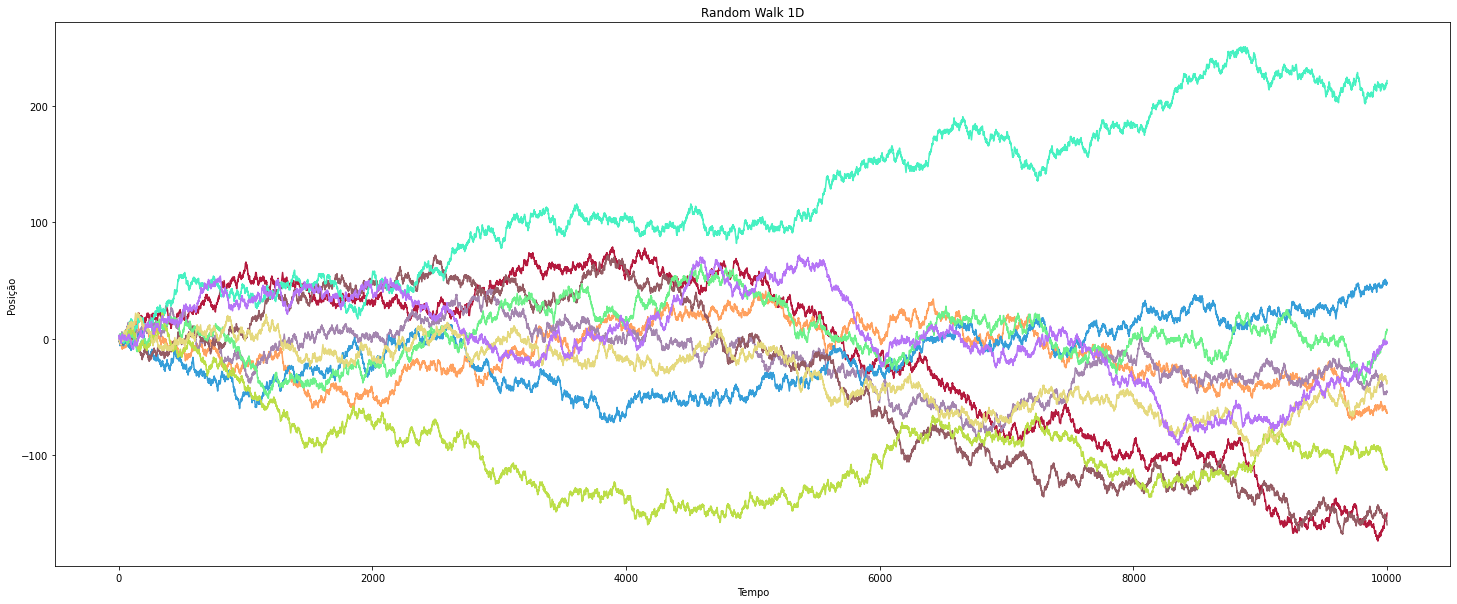
\includegraphics[width=1\textwidth]{figuras/output_0.png}
\end{figure}

Calculamos o desvio médio quadrático $R^{2}$ para todos os 10 caminhantes e desenhamos um gráfico com a escala log-log. 

\begin{figure}[!htb]
  \centering
  \caption{Desvio médio quadrático log-log}
  \label{devio_medio}
  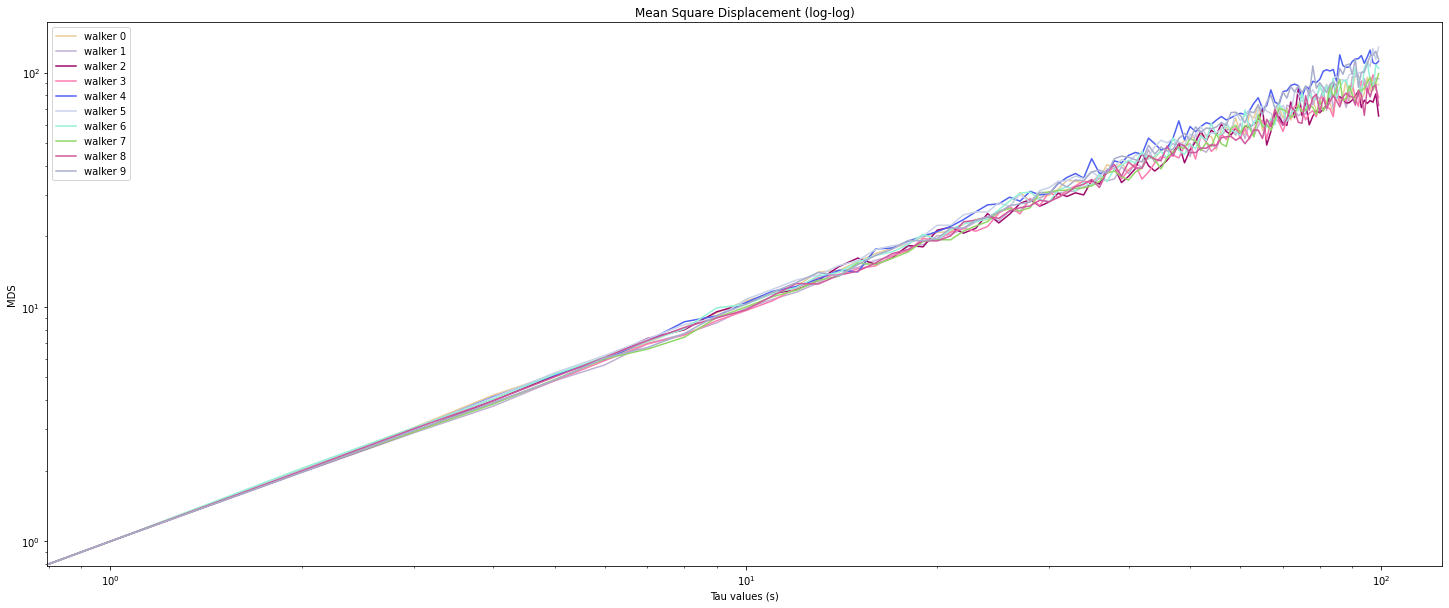
\includegraphics[width=1\textwidth]{figuras/output_1.png}
\end{figure}

Para ter uma série de dados única para ajustar uma função de lei de potência, fizemos a média dos resultados obtidos do $R^{2}$ de todos os caminhantes. A curva das médias pode ser vista no gráfico abaixo.

\begin{figure}[!htb]
  \centering
  \caption{Média do desvio médio quadrático log-log}
  \label{media_devio_medio}
  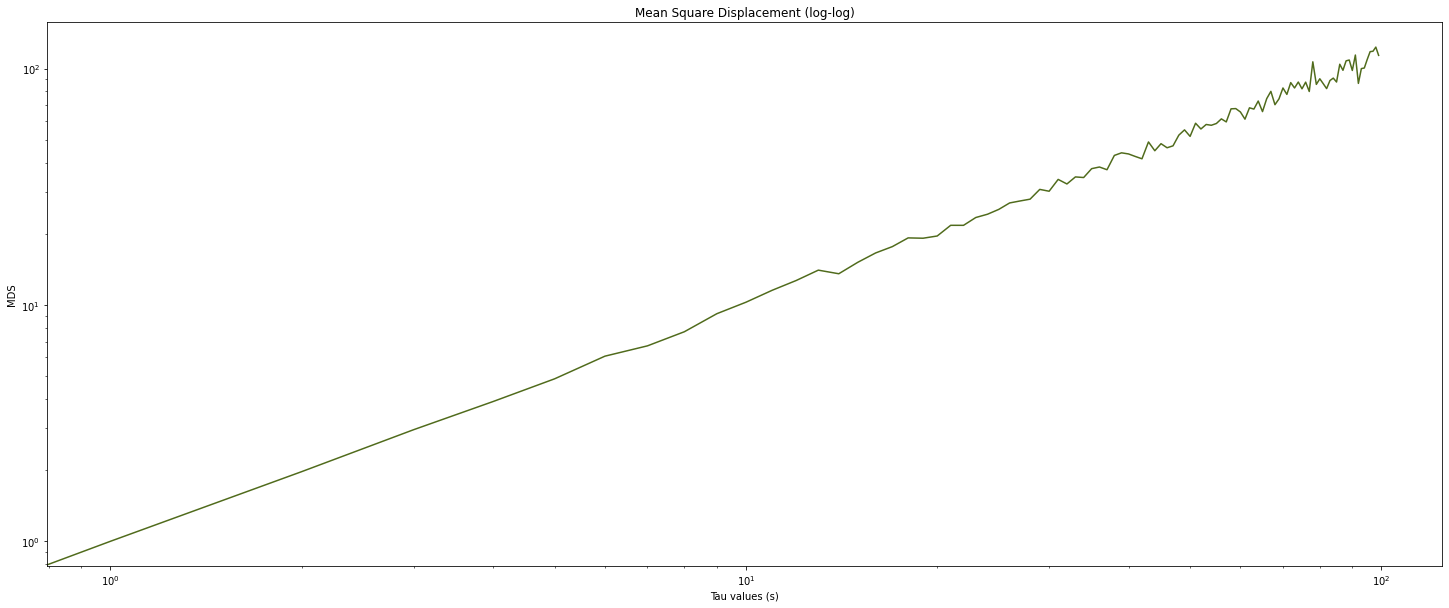
\includegraphics[width=1\textwidth]{figuras/output_2.png}
\end{figure}

Ajustamos a uma função de lei de potência para a série de dados e obtemos uma função com parâmetros:
$ a: 1.0632266820499991 $ e $ b: 0.9836350285341431 $. 

$$ y = 1.063226682049999x^{0.9836350285341431} $$

Desenhamos um novo gráfico com a serie de dados e com a função da lei de potência para visualizar a qualidade do ajuste.

\begin{figure}[!htb]
  \centering
  \caption{Lei de potência}
  \label{curva_lei_potencia}
  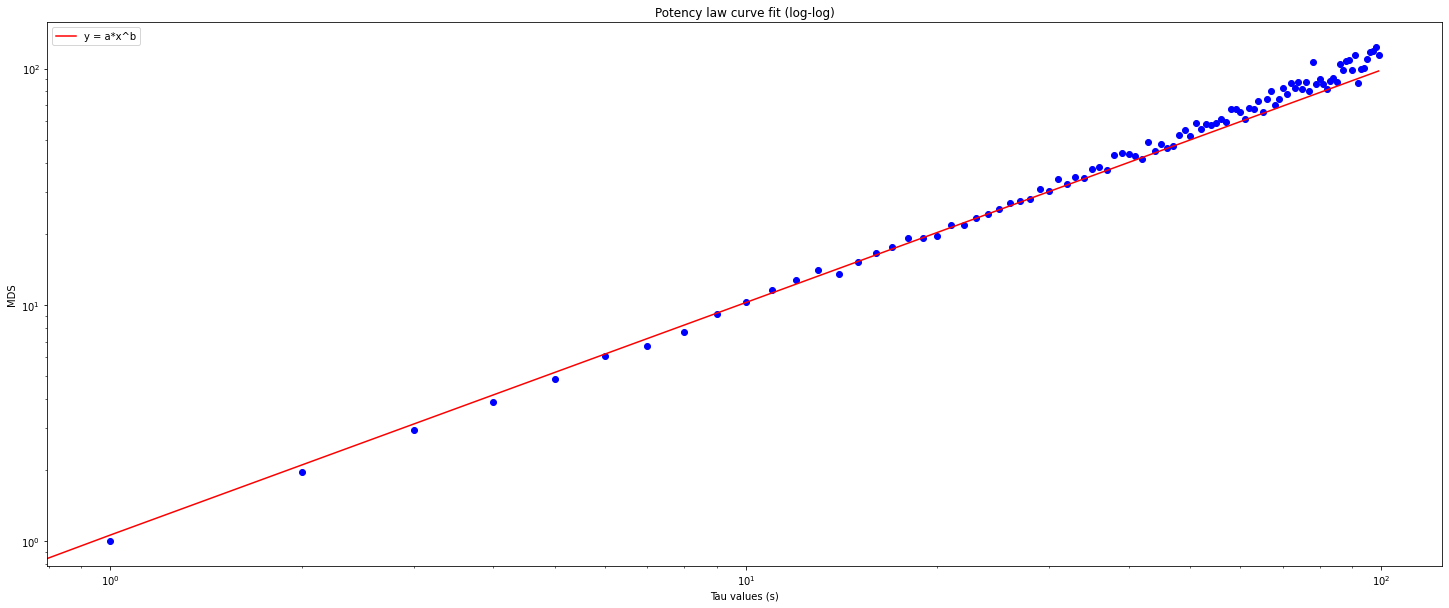
\includegraphics[width=1\textwidth]{figuras/output_3.png}
\end{figure}

Para verificar que a simulação respeita o teorema central do limite, desenhamos um histograma com a posição final de 1000 caminhantes e utilizamos o histograma para ajustar uma função gaussiana. O gráfico abaixo mostra o resultado obtido. 

\begin{figure}[!htb]
  \centering
  \caption{Histograma}
  \label{histograma}
  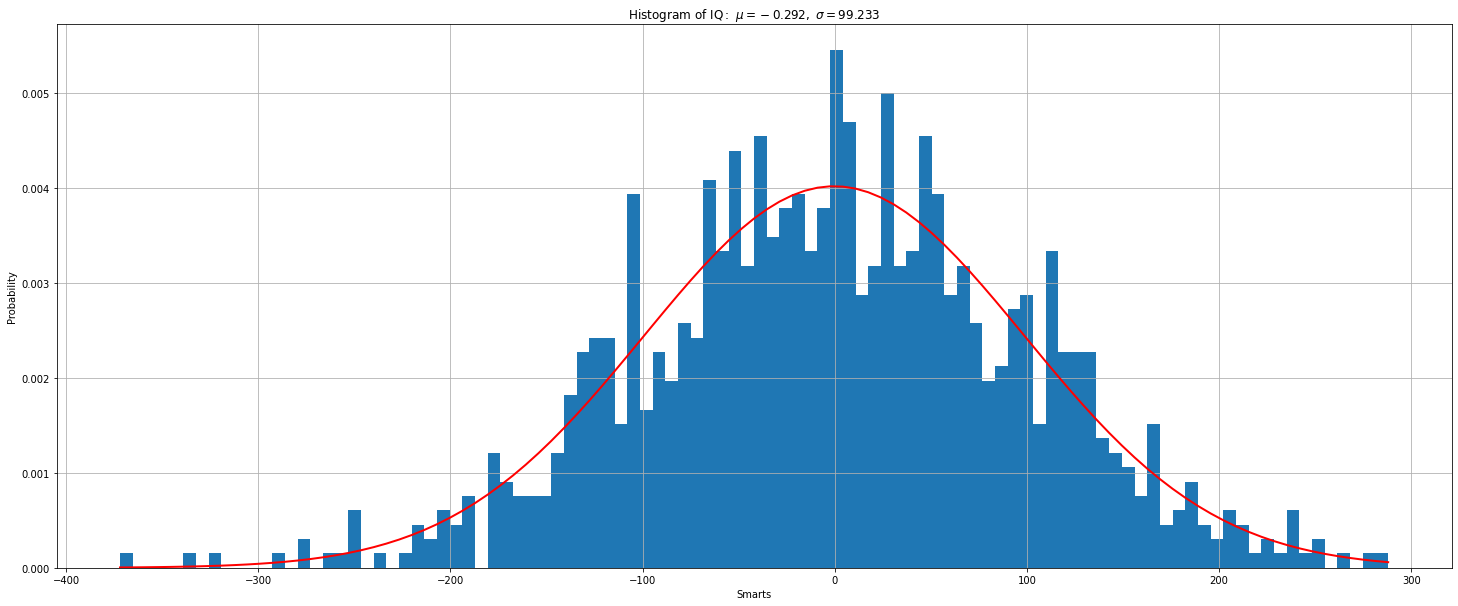
\includegraphics[width=1\textwidth]{figuras/output_4.png}
\end{figure}

\section{Discussão}
\label{sec_discussao_resultados}

O gráfico de posição x tempo é uma ótima forma de visualizar comparativamente as diversas interações da simulação do random walk. Com ele podemos visualizar lado a lado a posição de cada simulação desde a origem até a posição final. O formato final das curvas nos permite adquirir a intuição sobre o comportamento de uma entidade se movendo de maneira aleatória.

Ao calcular o desvio médio quadrático e desenhar o gráfico na escala log-log. Vemos que as curvas são aproximadamente lineares. os gráfico log-log mostram linhas retas para funções exponenciais, variando a inclinação da reta de acordo com o expoente. 

Para identificar o expoente da função fazemos o ajuste de uma função de lei de potência. A função ajustada tem expoente 1, o que indica que o random walk implementado é realmente um caminhante aleatório.

O gráfico da função ajustada e da série de dados mostra que o ajuste feito realmente aproxima os valores da série.

O gráfico do histograma mostra o resultado da posição final de 1000 simulação. A posição final foi agrupada em blocos de 100 para cada coluna do histograma. Sobre o histograma desenhamos uma gaussiana (curva em formato de sino). Foi necessário normalizar o histograma antes de ajustar a gaussiana ajustada.
               % Resultados
% ------------------------------------------------------------------------------
% Conclusão
% ------------------------------------------------------------------------------

\chapter{Conclusão}
\label{chap_conclusao}

O experimento mostrou que o algoritmo random walk utilizando um gerador de números aleatórios congruencial realmente gerou um caminhante aleatório. Conseguimos confirmar isso ao observar que o expoente da função da lei de potência ajustada tem expoente 1, indicando que a partícula em movimento não está confinada nem se movendo dentro de um fluxo de força externo.

O histograma desenhado com a posição final do caminhante mostra claramente que a distribuição de dados tem o formato de uma gaussiana. Ou seja, a distribuição de frequência da posição final do random walk respeita o teorema central do limite.

\section{Trabalhos futuros}
\label{sec_trabalhos_futuros}

Nesse trabalho exploramos o random walk apenas uma dimensão. Fazer simulações em mais dimensões e avaliar se as propriedades observadas serão as mesmas é uma maneira de dar continuidade a esse trabalho.  

% ------------------------------------------------------------------------------
% Observação: A norma ABNT estabelece que, em qualquer categoria de trabalho
% acadêmico monográfico deve haver um capítulo de conclusão
% ------------------------------------------------------------------------------
                % Conclusão

\postextual % Define o estilo de página para os elementos pós-textuais

\imprimirreferencias{referencias.bib}                   % Referências
%% ------------------------------------------------------------------------------
% Apêndices
% ------------------------------------------------------------------------------

\begin{apendicesenv}
    \partapendices

    % --------------------------------------------------------------------------
    % Primeiro apêndice
    % --------------------------------------------------------------------------

    \chapter{Nome do apêndice}
    \label{chap_apendice_a}

    Lembre-se que a diferença entre apêndice e anexo diz respeito à autoria do texto e/ou material ali colocado.

    Caso o material ou texto suplementar, ou complementar seja de sua autoria, então ele deverá ser colocado como um apêndice.
    Porém, caso a autoria seja de terceiros, então o material ou texto deverá ser colocado como anexo.

    Caso seja conveniente, podem ser criados outros apêndices para o seu trabalho acadêmico.
    Basta recortar e colar este trecho neste mesmo documento.

\end{apendicesenv}            % Apêndices
%% ------------------------------------------------------------------------------
% Anexos
% ------------------------------------------------------------------------------

\begin{anexosenv}
    \partanexos

    % --------------------------------------------------------------------------
    % Primeiro anexo
    % --------------------------------------------------------------------------

    \chapter{Nome do anexo}
    \label{chap_anexo_a}

    Lembre-se que a diferença entre apêndice e anexo diz respeito à autoria do texto e/ou material ali colocado.

    Caso o material ou texto suplementar, ou complementar seja de sua autoria, então ele deverá ser colocado como um apêndice.
    Porém, caso a autoria seja de terceiros, então o material ou texto deverá ser colocado como anexo.

    Caso seja conveniente, podem ser criados outros anexos para o seu trabalho acadêmico.
    Basta recortar e colar este trecho neste mesmo documento.

    Organize seus anexos de modo que, em cada um deles, haja um único tipo de conteúdo.
    Isso facilita a leitura e compreensão para o leitor do trabalho. É para ele que você escreve.

\end{anexosenv}
               % Anexos
\printindex                                             % Índice remissivo

\end{document}
